\documentclass[12pt]{article}
\usepackage{graphicx}
\usepackage{float}
\usepackage{hyperref}
\usepackage{tfrupee}
\usepackage{ragged2e}
\usepackage{multicol}
\usepackage{multirow}
\usepackage{xurl}
\usepackage{geometry}
\usepackage{enumitem}
\documentclass{minimal}
\usepackage{mathtools}
\DeclarePairedDelimiter\ceil{\lceil}{\rceil}
\DeclarePairedDelimiter\floor{\lfloor}{\rfloor}
 \geometry{
 a4paper,
 total={170mm,240mm},
 left=20mm,
 top=20mm,
 }
% begin the document.
\begin{document}

% make a title page.[this creates title page]
\begin{center}\textbf{
\LARGE{EE338 : Digital Signal Processing}\\\vspace{1em}
\vspace{1em} \\ 
\LARGE{Filter Design Assignment}\\
\vspace{1em}
\large{February 27, 2023}\\
\vfill
\begin{figure}[H]
    \centering
    \includegraphics[scale = 0.2]{logo.png}
\end{figure}
\vspace{1em}
\large{Indian Institute of Technology, Bombay}\\
\vfill
\LARGE{Amruta Mahendra Parulekar} \\
\LARGE{Roll no. 20d070009} \vspace{2em}
\\\large{Reviewed by Sameep Chattopadhyay, 20d070067}

}
\end{center}

\newpage
\tableofcontents
\newpage
\section{Student Details} %[This segment creates Section as seen in document]
\begin{itemize}[nolistsep]
    \item Name = Amruta Mahendra Parulekar
    \item Roll no. = 20d070009
    \item Filter number m = 26
    \item Group number = 3
    \item Review member = Sameep Chattopadhyay, 20d070067 (Has reviewed my report)
\end{itemize}
\section{Butterworth filter Design}
\subsection{Un-normalized discrete time filter specifications}

  
    The filter to be designed is a Band-pass filter where:
    \begin{equation}
        q(m) = \floor{m/10} = \floor{2.6} = 2
    \end{equation}
    \begin{equation}
        r(m) = 26 - 10*q(m) = 26 - 10*2 = 6
    \end{equation}
    \begin{equation}
        BL(m) = 10 + 5*q(m) + 13*r(m) = 10 + 5*2 + 13*6 = 98
    \end{equation}
    \begin{equation}
        BH(m) = BL(m) + 75 = 98 + 75 = 173
    \end{equation}
  

    \begin{enumerate}
    \item \textbf{The passband will be monotonic and the stopband will be monotonic}
    \item \textbf{The passband will be from 98 kHz to 173 kHz}
    \item \textbf{The transition band will be 5 kHz on either side of the passband}
    \item \textbf{The stopband will be from 0 - 93 kHz and 178 - 300kHz} ( sampling rate 600 kHz)
    \item \textbf{The passband and stopband tolerances are 0.15 in magnitude}

\end{enumerate}
\subsection{Normalized discrete time filter specifications}
Sampling rate is 600 kHz, which corresponds to 2$\pi$ on the normalized frequency axis.
\\So on normalizing the frequency axis, each frequency $\Omega_1$ below 300 kHz gets mapped using the function:
\begin{equation}
    \omega=\frac{\Omega_1 * 2 \pi}{(Sampling Rate)}
\end{equation}
\begin{enumerate}
    \item \textbf{The passband will be monotonic and the stopband will be monotonic}
    \item \textbf{The passband will be from 0.3267 $\pi$ to 0.5767 $\pi$}
    \item \textbf{The transition band will be 0.017 $\pi$ on either side of the passband}
    \item \textbf{The stopband will be from 0 $\pi$ - 0.31 $\pi$ and 0.593 $\pi$- $\pi$}
    \item \textbf{The passband and stopband tolerances are 0.15 in magnitude}

\end{enumerate}
\newpage
\subsection{Analog filter specifications }
The discrete time filter specifications can be converted to corresponding analog filter specifications by using a bilinear transform, which is given as:
\begin{equation}
    \Omega = tan(\omega/2)
\end{equation}
\begin{enumerate}
    \item \textbf{The passband will be monotonic and the stopband will be monotonic}
    \item \textbf{The passband will be from 0.5635($\Omega_{p1}$) to 1.2754($\Omega_{p2}$)}
    \item \textbf{The transition band will be from 0.5295($\Omega_{s1}$) - 0.5635($\Omega_{p1}$) and \\from 1.2754($\Omega_{p2}$)-1.345($\Omega_{s2}$)}
    \item \textbf{The stopband will be from 0 - 0.5295($\Omega_{s1}$) and 1.345($\Omega_{s2}$) - infinity}
    \item \textbf{The passband and stopband tolerances are 0.15 in magnitude}

\end{enumerate}
\subsection{The frequency transformation }
We use the bandpass transformation to convert the band pass filter to a lower filter:
\begin{equation}
    \Omega_L=\frac{\Omega^2-\Omega_{0}^2}{B\Omega}
\end{equation}
The two parameters B and $\Omega_{0}$ are obtained by the relations:
\begin{equation}
    \Omega_{0}=\sqrt{\Omega_{p1}*\Omega_{p2}}= \sqrt{0.5635*1.2753}=0.8478
    \end{equation}
    \begin{equation}   
    B=\Omega_{p2}-\Omega_{p1}=0.7118
 \end{equation}
 \begin{center}
\def\arraystretch{1.1}
\bgroup
\begin{tabular}{|c|c|}
\hline
\textbf{$\Omega$ }
& \textbf{$\Omega_L$ }\\ 
\hline \hline
$0^+$  &  -infinity  \\ 
\hline 
0.5295 ($\Omega_{s1}$)   &   -1.163 ($\Omega_{Ls1}$) \\ 
\hline
 0.5635 ($\Omega_{p1}$) &    -1 ($\Omega_{Lp1}$)\\ 
\hline
0.8478  ($\Omega_{0}$) & 0  \\ 
\hline
1.2753 ($\Omega_{p2}$)   &  1 ($\Omega_{Lp2}$) \\ 
\hline
 1.345 ($\Omega_{s2}$) &   1.139 ($\Omega_{Ls2}$) \\ 
 \hline
 infinity & infinity \\
 \hline
\end{tabular}
\egroup
\end{center}
\subsection{Frequency transformed lowpass analog filter specifications}
\begin{enumerate}
    \item \textbf{The passband will be monotonic and the stopband will be monotonic}
    \item \textbf{The passband edge will be at 1($\Omega_{Lp}$)}
    \item \textbf{The stopband edge will be min(-$\Omega_{Ls1}$,$\Omega_{Ls2}$) which is 1.139($\Omega_{Ls}$)}
    \item \textbf{The passband and stopband tolerances are 0.15 in magnitude}

\end{enumerate}
\newpage
\subsection{The analog lowpass filter transfer function}
We require a Butterworth Bandpass filter, which means that both the passband and stopband are monotonic.
\\Since the tolerance ($\delta$) in both passband and stopband is 0.15, we define :
\begin{equation}
    D1= \frac{1}{(1-\delta)^2}-1 = 0.3841
\end{equation}
\begin{equation}
    D2= \frac{1}{(\delta)^2}-1 = 43.444
\end{equation}
The inequality for the order N of the Butterworth filter is:
\begin{equation}
    N_{min}=\ceil{\frac{log(\sqrt{D2/D1})}{log(\Omega_{Ls}/\Omega_{Lp})}} = 19
\end{equation}
The inequality for the cutoff frequency $\Omega_{c}$ of the Analog lowpass filter is:
\begin{equation}
   \frac{ \Omega_{Lp}}{D_1^{1/2N}} \leq \Omega_{c} \leq \frac{ \Omega_{Ls}}{D_2^{1/2N}}
\end{equation}
\begin{equation}
   1.0255 \leq \Omega_{c} \leq 1.0317
\end{equation}
So we take average $\Omega_{c} = 1.0286$
\\The poles of the transfer function can be obtained by solving:
\begin{equation}
   1+ (\frac{s}{j\Omega_{c}})^{2N} = 1+ (\frac{s}{j1.0286})^{38} = 0
\end{equation}
On plotting the above equation, we get the location of the roots using Wolfram alpha as shown:
\begin{figure}[H]
    \centering
    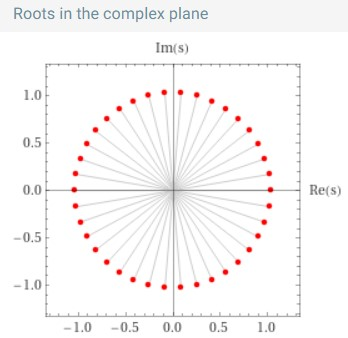
\includegraphics[]{poles.jpg}
\end{figure}

The poles obtained are symmetric about the origin and we can pick one from each pair for our transfer function. We choose poles from the LHCP to allow stability. 
\newpage
Apart from -1.086 which is the real pole, the poles chosen are:
\begin{figure}[H]
    \centering
    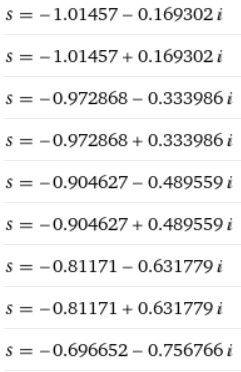
\includegraphics[]{roots.jpg}
    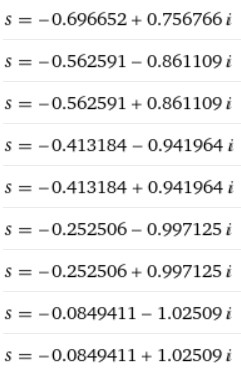
\includegraphics[]{r2.jpg}
\end{figure}
We can write the transfer function as:
\begin{equation}
    H_{analog,LPF}(s_L)=\frac{\Omega_{c}^N}{\prod_{i=1}^{N}(s_L-p_i)} = \frac{1.709}{\prod_{i=1}^{19}(s_L-p_i)}
\end{equation}
The numerator has been scaled to get a DC gain of 1.
\subsection{The analog bandpass filter transfer function}
The transformation equation:
\begin{equation}
    s_L= \frac{s^2+\Omega_{0}^2}{Bs} = \frac{s^2+0.8478^2}{0.7118*s}
\end{equation}
Thus, the transfer function:
\begin{equation}
    H_{analog,BPF}(s)=\frac{\Omega_{c}^{19}(Bs)^{19}}{\prod_{i=0}^{18}(s^2-p_iBs+\Omega_{0}^2)} 
\end{equation}
Factorizing the denominator to get new roots so that the denominator can be expressed as a product of 38 monomials, we get the new poles as:
\begin{equation}
    pol_i=\frac{p_iB\pm \sqrt{(p_iB)^2+4\Omega_{0}^4}}{2}
\end{equation}
Thus the new analog filter transfer function where $pol_i$ are poles of the analog bandpass filter is:
\begin{equation}
    H_{analog,BPF}(s)=\frac{\Omega_{c}^{19}(Bs)^{19}}{\prod_{i=0}^{37}(s-pol_i)} 
\end{equation}
\newpage
The transfer function and its coefficients after expansion can be seen as:
\\\textbf{Numberator:}0.00267*x**19
\\\textbf{Denominator}
    x**38 + 8.8661*x**37 - 1.5913e-8*I*x**37 + 52.9604*x**36 - 1.4109e-7*I*x**36 + 230.3324*x**35 - 8.2849e-7*I*x**35 + 821.3392*x**34 - 3.5385e-6*I*x**34 + 2466.2229*x**33 - 1.2328e-5*I*x**33 + 6460.0678*x**32 - 3.6087e-5*I*x**32 + 14961.5867*x**31 - 9.1846e-5*I*x**31 + 31125.4114*x**30 - 0.0002*I*x**30 + 58616.1143*x**29 - 0.0004*I*x**29 + 100785.1822*x**28 - 0.0007*I*x**28 + 158973.7331*x**27 - 0.0012*I*x**27 + 231217.9001*x**26 - 0.00188*I*x**26 + 311017.9860*x**25 - 0.0026*I*x**25 + 388150.0445*x**24 - 0.0033*I*x**24 + 450252.6990*x**23 - 0.0039*I*x**23 + 486414.6177*x**22 - 0.0043*I*x**22 + 489860.0993*x**21 - 0.0044*I*x**21 + 460388.8194*x**20 - 0.0042*I*x**20 + 403908.1601*x**19 - 0.0036*I*x**19 + 330911.2961*x**18 - 0.0030*I*x**18 + 253072.9427*x**17 - 0.0022*I*x**17 + 180620.5212*x**16 - 0.0016*I*x**16 + 120172.0923*x**15 - 0.0010*I*x**15 + 74461.8398*x**14 - 0.0006*I*x**14 + 42885.1024*x**13 - 0.0003*I*x**13 + 22915.4939*x**12 - 0.0001*I*x**12 + 11324.5243*x**11 - 8.8595e-5*I*x**11 + 5160.3374*x**10 - 3.8530e-5*I*x**10 + 2157.1744*x**9 - 1.5255e-5*I*x**9 + 823.3228*x**8 - 5.4538e-6*I*x**8 + 284.4589*x**7 - 1.7462e-6*I*x**7 + 88.2807*x**6 - 4.9315e-7*I*x**6 + 24.2241*x**5 - 1.2109e-7*I*x**5 + 5.7986*x**4 - 2.4982e-8*I*x**4 + 1.1688*x**3 - 4.2041e-9*I*x**3 + 0.1931*x**2 - 5.1461e-10*I*x**2 + 0.0232*x - 4.1719e-11*I*x + 0.0018
    \\(Where I refers to iota and ** refers to powers of x)
\subsection{The discrete time filter transfer function}
The bilinear transform from analog to discrete domain is:
\begin{equation}
    \frac{1-z^{-1}}{1+z^{-1}}
\end{equation}
On substituting this s in equation for the analog Bandpass filter, we get:
\begin{equation}
    H_{discrete,BPF}(s)=\frac{\Omega_{c}^{19}(B)^{19}(1-z^{-2})^{19}}{\prod_{i=0}^{37}((1-pol_i)-(1+pol_i)z^{-1})} 
\end{equation}
Thus we get new the poles at:
\begin{equation}
    z_i=\frac{1+pol_i}{1-pol_i}
\end{equation}
Since we have $p_i$ values for the analog lowpass filter, we can use equation (19) to get $pol_i$ values for the poles of the analog bandpass filter. 
\\Once we have the  $pol_i$ values for the poles of the analog bandpass filter, we can use equation (23) to compute the poles of the discrete bandpass filter. 
\\We have the values of all coefficients for equation (22) and thus we can substitute and find the values of the coefficients of the discrete bandpass filter transfer function.
\vfill
\begin{center}
    

\textbf{THUS THE BUTTERWORTH IIR FILTER DESIGN ASSIGNMENT HAS BEEN COMPLETED.}
\end{center}
\newpage
\section{Plots}

    
\subsection{The frequency vs magnitude plot:}Here, we can see the values 0.5295 ($\Omega_{s1}$); 0.5635 ($\Omega_{p1}$); 1.2753 ($\Omega_{p2}$); 1.345 ($\Omega_{s2}$) very clearly.
\begin{center}
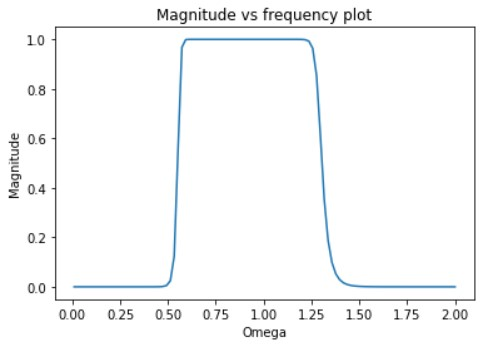
\includegraphics[]{plot1.jpg}
\end{center}
\subsection{The magnitude(log) and phase response of the filter:}
\begin{center}
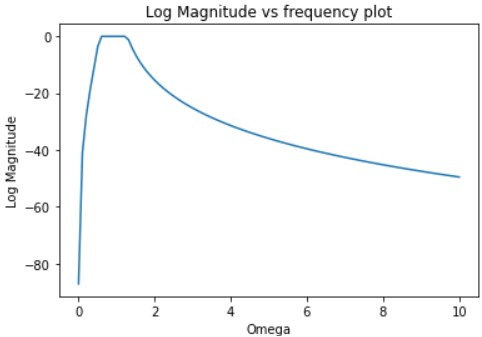
\includegraphics[scale=0.8]{plot2.jpg}
\\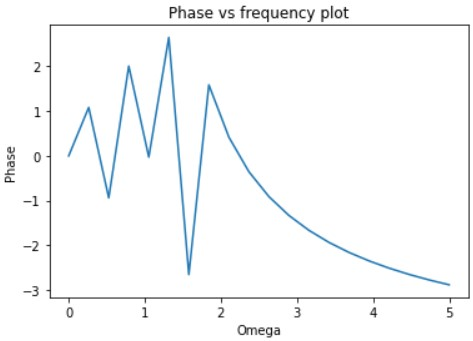
\includegraphics[scale=0.8]{freqplot.jpg}
\end{center}
\section{Code}
\subsection{Code for evaluating the analog filter response:}
\begin{center}
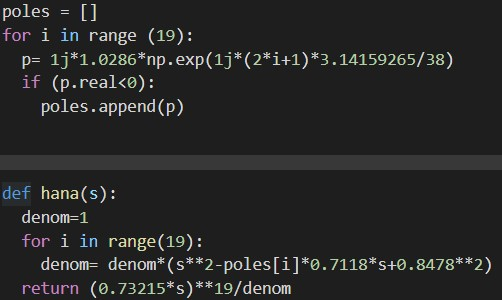
\includegraphics[]{code for plot1.jpg}

\end{center}
\subsection{Code for plots:}
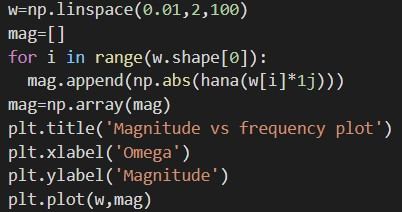
\includegraphics[]{code for plot2.jpg}
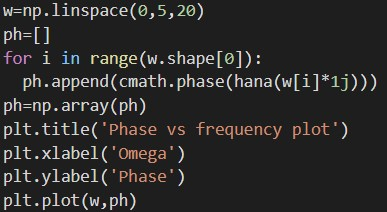
\includegraphics[]{code for plot3.jpg}
\subsection{Code for printing denominator coefficients:}
\begin{center}
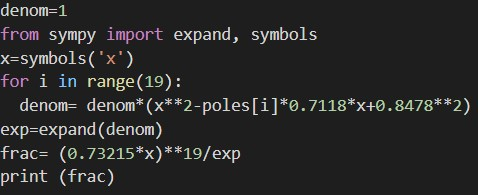
\includegraphics[scale=0.9]{code .jpg}
\end{center}
\section{Peer Review}
\textbf{I have reviewed the report of Harshvardhan (20d070035) and have found it to be correct.} The filter design steps were completed and the phase and magnitude response plots were present. He has started from the un-normalised filter, then normalized it, then converted to an analog filter, which was converted to a lowpass filter, to which he applied a frequency transform and then reconverted it to a bandpass filter.

\end{document}
